\documentclass[11pt, a4paper]{article}
\usepackage{graphicx}
\usepackage{amsmath}
\usepackage[margin=0.8in]{geometry}
\usepackage{listings}
\usepackage{float}
\usepackage{indentfirst}
\usepackage[inline]{enumitem}
\usepackage{tabularx}
\usepackage{xcolor}
\usepackage{array}
\usepackage{minted}
\usemintedstyle{vs}
\usepackage[belowskip=0pt,aboveskip=0pt,font=small,labelfont=small]{caption}


\title{EE2703: Assignment 7: The Laplace Transform}
\author{Sakthi Harish D T (EE19B054)}
\date{April $16^{th}$, 2021}

\begin{document}
\maketitle
\section{Abstract:}
In this assignment, we will,
\begin{enumerate}
    \item solve for the time response of a spring with different decays and frequencies
    \item solve for a coupled spring problem
    \item obtain the magnitude and phase response of the Steady State Transfer function of a two-port network
    \item obtain the $v_o(t)$ for the said two-port network
\end{enumerate}
\section{Introduction:}
    In this assignment, we will make use of Laplace Transform to solve 
    'continuous time' systems. We will analyse the LTI systems using the python library, \texttt{scipy.signal}. 

\section{Time Response of a Spring:}
    We need to find the response of a spring, whose equation is given by,
    \begin{equation*}
        \ddot{x} + 2.25x = f(t)
    \end{equation*}
    Here f(t) is given by,
    \begin{equation*}
        f(t) = e^{-at}cos(\omega t)u(t)
    \end{equation*}
    where, $'a'$ represents decay and takes values 0.5 and 0.05. $\omega$ takes values 1.4, 1.45, 1.5, 1.55 and 1.6 . \newline
    We will use the \textbf{Laplace Transform} to solve the problem.\newline
        The Laplace transform of $f(t) = e^{-at}cos(\omega t)u(t)$ is given as:
        \begin{equation*}
            \mathcal{L}\{f(t)\} = \frac{s+a}{(s+a)^2 + \omega^2}
        \end{equation*}

        From the property of Laplace transforms, we know:
        \begin{gather*}
            x(t) \longleftrightarrow \mathcal{X}(s)\\
            \implies \dot{x}(t) \longleftrightarrow \ s\mathcal{X}(s) - x(0^-)\\
            \implies \ddot{x}(t) \longleftrightarrow \ s^2\mathcal{X}(s) - sx(0^-)-\dot{x}(0^-)
        \end{gather*}

        From the above equations, we get, for $a = 0.5$ and $\omega = 1.5$:
        \begin{equation*}
            F(s) = \frac{s+0.5}{(s+0.5)^2+2.25}
        \end{equation*}

        Substituting the given ICs $x(0)$ and $\dot{x}(0)$ are 0, we get:

        \begin{equation*}
            X(s) = \frac{s+0.5}{((s+0.5)^2+2.25)(s^2+2.25)}
        \end{equation*}

        Using \texttt{scipy.signal.impulse} to find the x(t) by the following code, and plotting it (for $0<t<50 s$), we get:\newline
         \textit{\textbf{Python Code:}}
    \lstset{language=Python}
    \lstset{label={lst:code_direct}}
    \lstset{basicstyle=\footnotesize}
    \begin{lstlisting}
    F_num= np.poly1d([1, gamma1])      #defining numerator of function  with decay as 0.5 
    FX_den= np.polymul([1, 2*gamma1, gamma1**2 + w**2], [1, 0, 2.25])   
    X= sgnl.lti(F_num,FX_den)           
    t,x= sgnl.impulse(X, None, np.linspace(0, 50, 1000))    #Getting the solution for x(t)
    \end{lstlisting}
        \begin{figure}[H]
            \centering
            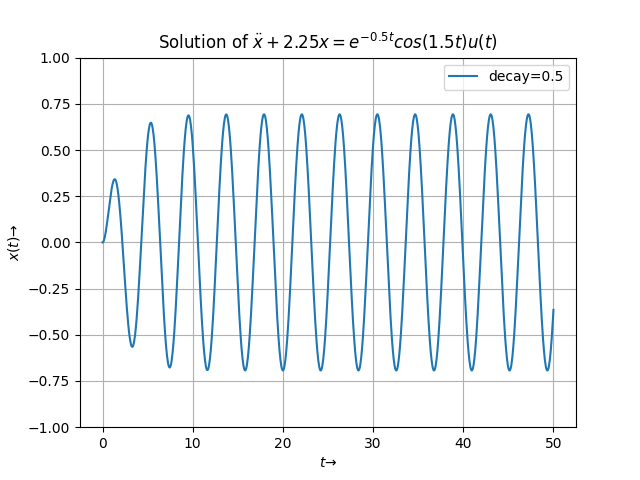
\includegraphics[scale=0.7]{Figure_1.png}
            \caption{$x(t)$ for $a=0.5$ and $\omega=1.5$}
            \label{fig:Fig1}
        \end{figure}

        Now, we use a smaller decay of $a=0.05$, we get:
        \begin{figure}[H]
            \centering
            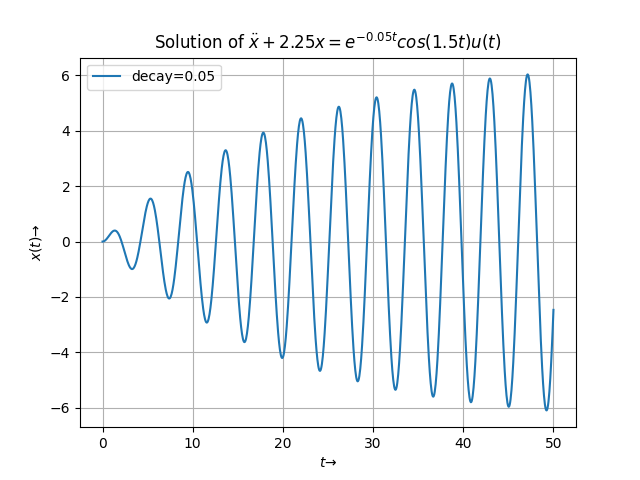
\includegraphics[scale=0.7]{Figure_2.png}
            \caption{$x(t)$ for $a=0.05$ and $\omega=1.5$}
            \label{fig:Fig2}
        \end{figure}
        Now, we obtain the response for different frequencies, using 
        \texttt{signal.lsim},\newline
                 \textit{\textbf{Python Code:}}
    \lstset{language=Python}
    \lstset{label={lst:code_direct}}
    \lstset{basicstyle=\footnotesize}
    \begin{lstlisting}
        H1_s = sgnl.lti([1], [1, 0, 2.25])        # Transfer function H1(s)= X(s)/F(s)
        plt.figure(3)                             
        for w in np.arange(1.4, 1.6, 0.05):     
            T = np.linspace(0, 50, 1000)
            t, y, rest = sgnl.lsim(H1_s,U= np.exp(-0.05*t)*np.cos(w*t), T=T)
            plt.plot(t,y, label='$w = {} rad/s$'.format(w))
            plt.legend()
        plt.grid()
        plt.show()
\end{lstlisting}

        \begin{figure}[H]
            \centering
            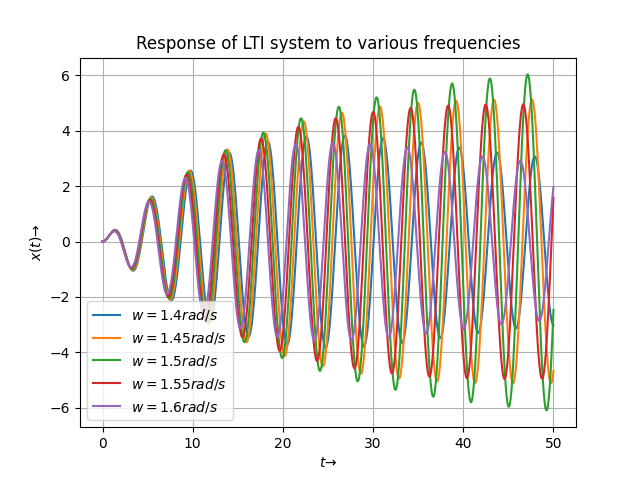
\includegraphics[scale=0.8]{Figure_3.png}
            \caption{$x(t)$ for $a=0.05$ and varying $\omega$}
            \label{fig:Fig3}
        \end{figure}
        We can see the maximum amplitude of oscillations is obtained when the frequency of $f(t)$ is $1.5\ rad/s$ . We can also see that
         $\omega= 1.5\ rad/s$ is the natural frequency. Therefore, at
          $\omega= 1.5\ rad/s$, it is in resonance.

\section{Coupled Spring Problem:}
    We have to solve the Coupled equations given by, 
    \begin{gather*}
        \ddot{x} + (x-y) = 0\\
        \ddot{y} + 2(y-x) = 0
    \end{gather*}

    Given the ICs $x(0)=1$ and $\dot{x}(0)=y(0)=\dot{y}(0)=0$. After solving ,we get the X(s) and Y(s) as,
    \begin{gather*}
        X(s) = \frac{s^2+3}{s^3+3s}\\
        Y(s) = \frac{2}{s^3+3s}
    \end{gather*}
    Now, we get the graph of x(t) and y(t) by using \texttt{signal.impulse} .
    \begin{figure}[H]
        \centering
        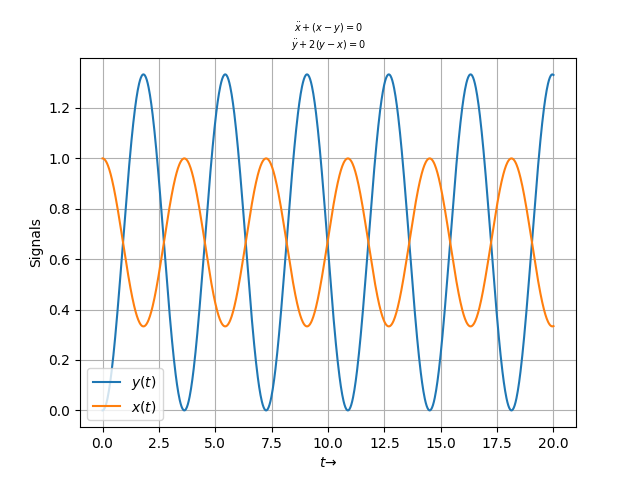
\includegraphics[scale=0.7]{Figure_4.png}
        \caption{$x(t)$ and $y(t)$ for the coupled spring problem}
        \label{fig:Fig4}
    \end{figure}

\section{Two-port Network:}
    The transfer function of the given two-port network can be written as:
    \begin{equation*}
        H(s)= \frac{V_o(s)}{V_i(s)} = \frac{1}{s^2LC+sRC+1}
    \end{equation*}

    The Bode magnitude and phase plots can be found using the method \texttt{scipy.signal.bode()}. The plots are shown below:
    \begin{figure}[H]
        \centering
        \setlength\tabcolsep{2pt}
        \begin{tabular}{cc}
            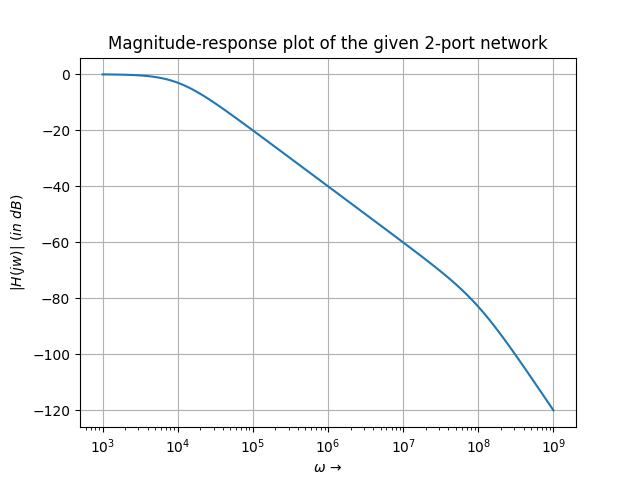
\includegraphics[scale=0.5]{Figure_5.png} &
            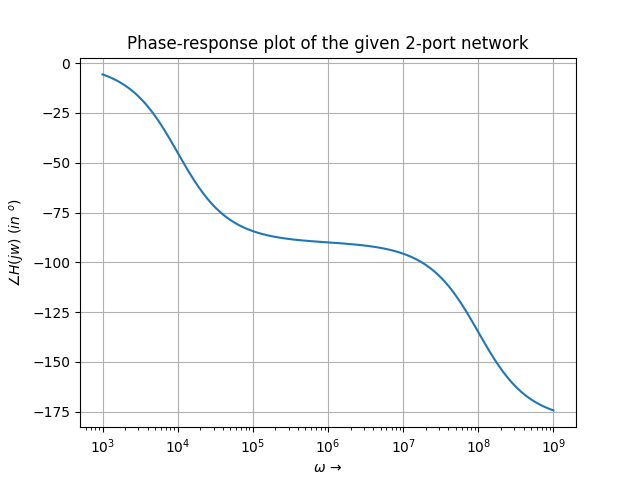
\includegraphics[scale=0.5]{Figure_6.png}\\
        \end{tabular}
        \caption{Bode Plots of the RLC Network's Transfer function}
    \end{figure}

    Now, when the input to the network, $v_i(t)$ is $cos(10^3t)u(t)-cos(10^6t)u(t)$, the output is given by:
    \begin{equation*}
        V_o(s) = V_i(s).H(s)
    \end{equation*}
    We will use \texttt{scipy.signal.lsim} to find $v_o(t)$ from $V_o(s)$.
    Plotting the obtained $v_o(t)$, we get:
    \begin{figure}[H]
        \centering
        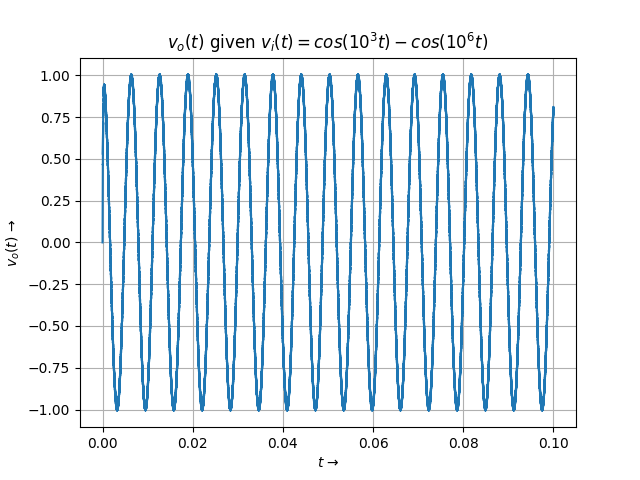
\includegraphics[scale=0.7]{Figure_7.png}
        \caption{$v_o(t)$ of the RLC network, when $v_i(t) = (cos(10^3t)-cos(10^6t))u(t)$}
        \label{fig:Fig6a}
    \end{figure}

    We can see it to be varying as a sinusoid of frequency approximately 160 Hz, which is expected, as the RLC network acts as a low pass filter - it allows low frequencies to pass through unchanged, while damping high frequencies to huge extent. 

    We notice that in the initial variation, When zoomed in, for $0<t<30\ us$, we get:
    \begin{figure}[H]
        \centering
        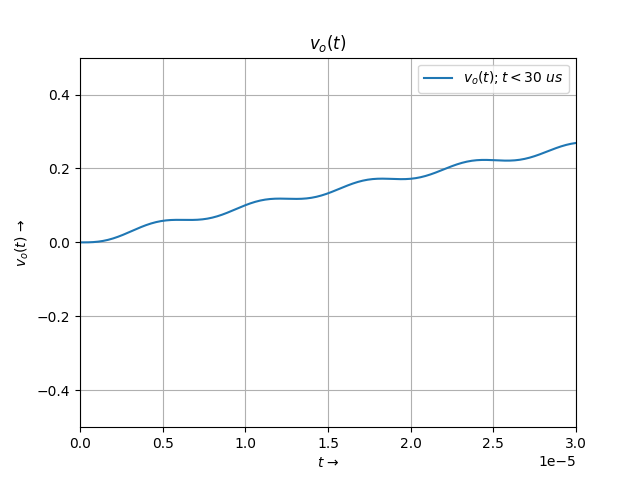
\includegraphics[scale=0.7]{Figure_8.png}
        \caption{Initial transients}
        \label{fig:Fig6b}
    \end{figure}

    This is due to application of the step input, i.e., the input is suddenly turned on at $t=0$.
\section{Conclusion}
In this assignment, we saw the power of Laplace Transform for the analysis of LTI systems. We used the \texttt{scipy.signal} python library
to obtain various signals from functions. We solved for the time response of a spring, coupled spring equations, and a two-port problem.
\end{document}

